\documentclass{article}\usepackage[]{graphicx}\usepackage[]{color}
%% maxwidth is the original width if it is less than linewidth
%% otherwise use linewidth (to make sure the graphics do not exceed the margin)
\makeatletter
\def\maxwidth{ %
  \ifdim\Gin@nat@width>\linewidth
    \linewidth
  \else
    \Gin@nat@width
  \fi
}
\makeatother

\definecolor{fgcolor}{rgb}{0.345, 0.345, 0.345}
\newcommand{\hlnum}[1]{\textcolor[rgb]{0.686,0.059,0.569}{#1}}%
\newcommand{\hlstr}[1]{\textcolor[rgb]{0.192,0.494,0.8}{#1}}%
\newcommand{\hlcom}[1]{\textcolor[rgb]{0.678,0.584,0.686}{\textit{#1}}}%
\newcommand{\hlopt}[1]{\textcolor[rgb]{0,0,0}{#1}}%
\newcommand{\hlstd}[1]{\textcolor[rgb]{0.345,0.345,0.345}{#1}}%
\newcommand{\hlkwa}[1]{\textcolor[rgb]{0.161,0.373,0.58}{\textbf{#1}}}%
\newcommand{\hlkwb}[1]{\textcolor[rgb]{0.69,0.353,0.396}{#1}}%
\newcommand{\hlkwc}[1]{\textcolor[rgb]{0.333,0.667,0.333}{#1}}%
\newcommand{\hlkwd}[1]{\textcolor[rgb]{0.737,0.353,0.396}{\textbf{#1}}}%

\usepackage{framed}
\makeatletter
\newenvironment{kframe}{%
 \def\at@end@of@kframe{}%
 \ifinner\ifhmode%
  \def\at@end@of@kframe{\end{minipage}}%
  \begin{minipage}{\columnwidth}%
 \fi\fi%
 \def\FrameCommand##1{\hskip\@totalleftmargin \hskip-\fboxsep
 \colorbox{shadecolor}{##1}\hskip-\fboxsep
     % There is no \\@totalrightmargin, so:
     \hskip-\linewidth \hskip-\@totalleftmargin \hskip\columnwidth}%
 \MakeFramed {\advance\hsize-\width
   \@totalleftmargin\z@ \linewidth\hsize
   \@setminipage}}%
 {\par\unskip\endMakeFramed%
 \at@end@of@kframe}
\makeatother

\definecolor{shadecolor}{rgb}{.97, .97, .97}
\definecolor{messagecolor}{rgb}{0, 0, 0}
\definecolor{warningcolor}{rgb}{1, 0, 1}
\definecolor{errorcolor}{rgb}{1, 0, 0}
\newenvironment{knitrout}{}{} % an empty environment to be redefined in TeX

\usepackage{alltt}
\IfFileExists{upquote.sty}{\usepackage{upquote}}{}
\begin{document}

\section{Data Description}

This data was collected on September 20, 2016 along 3 reaches of the Santa Ana River, with 9 observations per reach. Each observation contains the following variables:  

\subsection{Importing Data}

The following code was used to import data into rstudio, assign a file path, and create a command to read the csv file. 
\begin{knitrout}
\definecolor{shadecolor}{rgb}{0.969, 0.969, 0.969}\color{fgcolor}\begin{kframe}
\begin{alltt}
\hlstd{mydataGood}\hlkwb{=} \hlstr{"/home/CAMPUS/vesj2015/Santa-Ana-Sucker-Recovery/Data/Data_TUES_1/AllParametersGood.csv"}

\hlstd{importGood}\hlkwb{=}\hlkwd{read.csv}\hlstd{(mydataGood)}
\end{alltt}
\end{kframe}
\end{knitrout}
\subsection{Summary Statistics}

The following code was used to generate summary statisitics. 
\begin{knitrout}
\definecolor{shadecolor}{rgb}{0.969, 0.969, 0.969}\color{fgcolor}\begin{kframe}
\begin{alltt}
\hlkwd{summary}\hlstd{(importGood)}
\end{alltt}
\begin{verbatim}
##        ID       Site      Algae           Sediment       Temperature   
##  Min.   : 1.0   A:9   Min.   :  0.00   Min.   :0.0000   Min.   :28.00  
##  1st Qu.: 7.5   B:9   1st Qu.:  0.00   1st Qu.:0.0000   1st Qu.:29.00  
##  Median :14.0   C:9   Median : 50.00   Median :1.0000   Median :29.00  
##  Mean   :14.0         Mean   : 48.52   Mean   :0.5926   Mean   :28.89  
##  3rd Qu.:20.5         3rd Qu.:100.00   3rd Qu.:1.0000   3rd Qu.:29.00  
##  Max.   :27.0         Max.   :100.00   Max.   :1.0000   Max.   :30.00  
##      Canopy      
##  Min.   : 0.000  
##  1st Qu.: 3.000  
##  Median :11.000  
##  Mean   : 8.593  
##  3rd Qu.:14.000  
##  Max.   :15.000
\end{verbatim}
\end{kframe}
\end{knitrout}


\subsection{Distribution}

Write some stuff about the summary here...
\begin{knitrout}
\definecolor{shadecolor}{rgb}{0.969, 0.969, 0.969}\color{fgcolor}\begin{kframe}
\begin{alltt}
\hlkwd{hist}\hlstd{(importGood}\hlopt{$}\hlstd{Algae)}
\end{alltt}
\end{kframe}
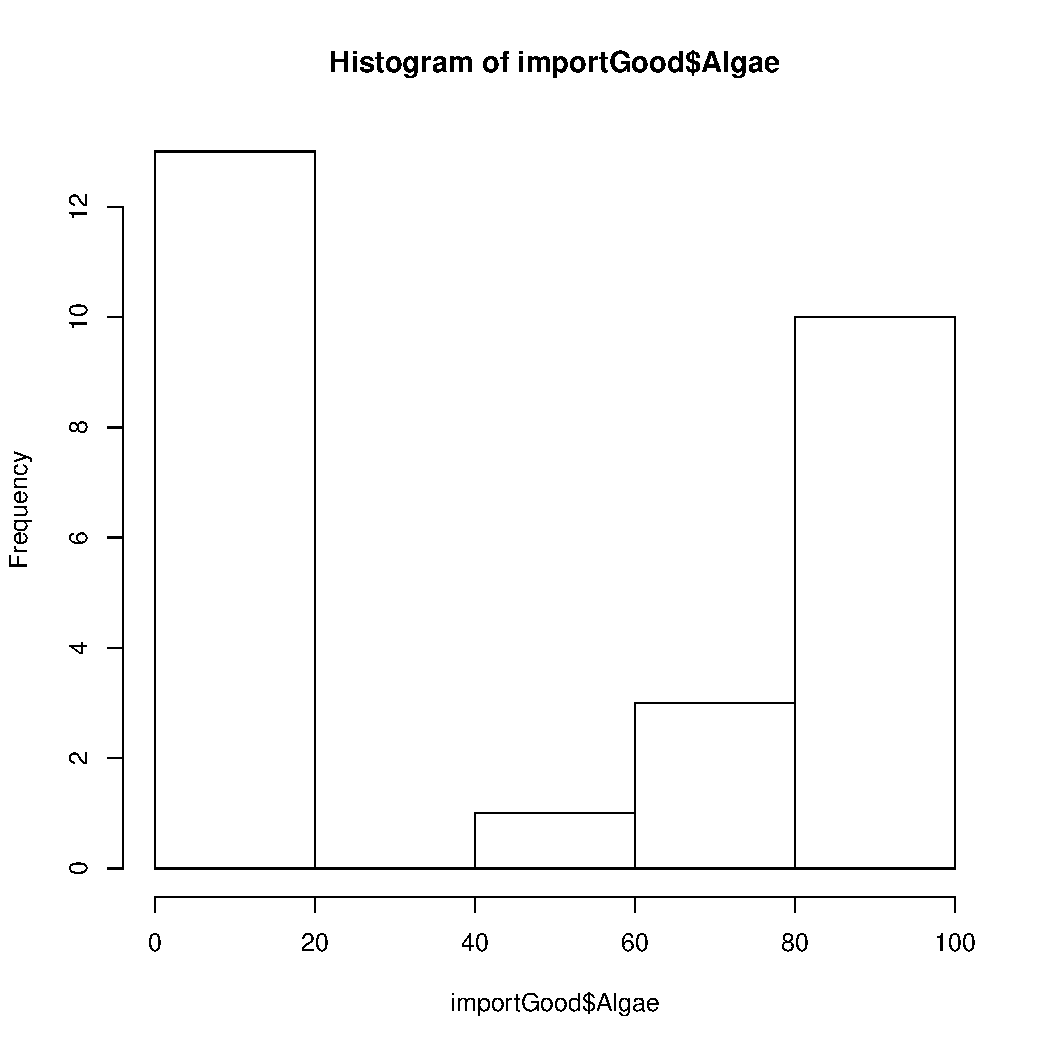
\includegraphics[width=\maxwidth]{figure/unnamed-chunk-3-1} 

\end{knitrout}

\begin{knitrout}
\definecolor{shadecolor}{rgb}{0.969, 0.969, 0.969}\color{fgcolor}\begin{kframe}
\begin{alltt}
\hlkwd{hist}\hlstd{(importGood}\hlopt{$}\hlstd{Sediment)}
\end{alltt}
\end{kframe}
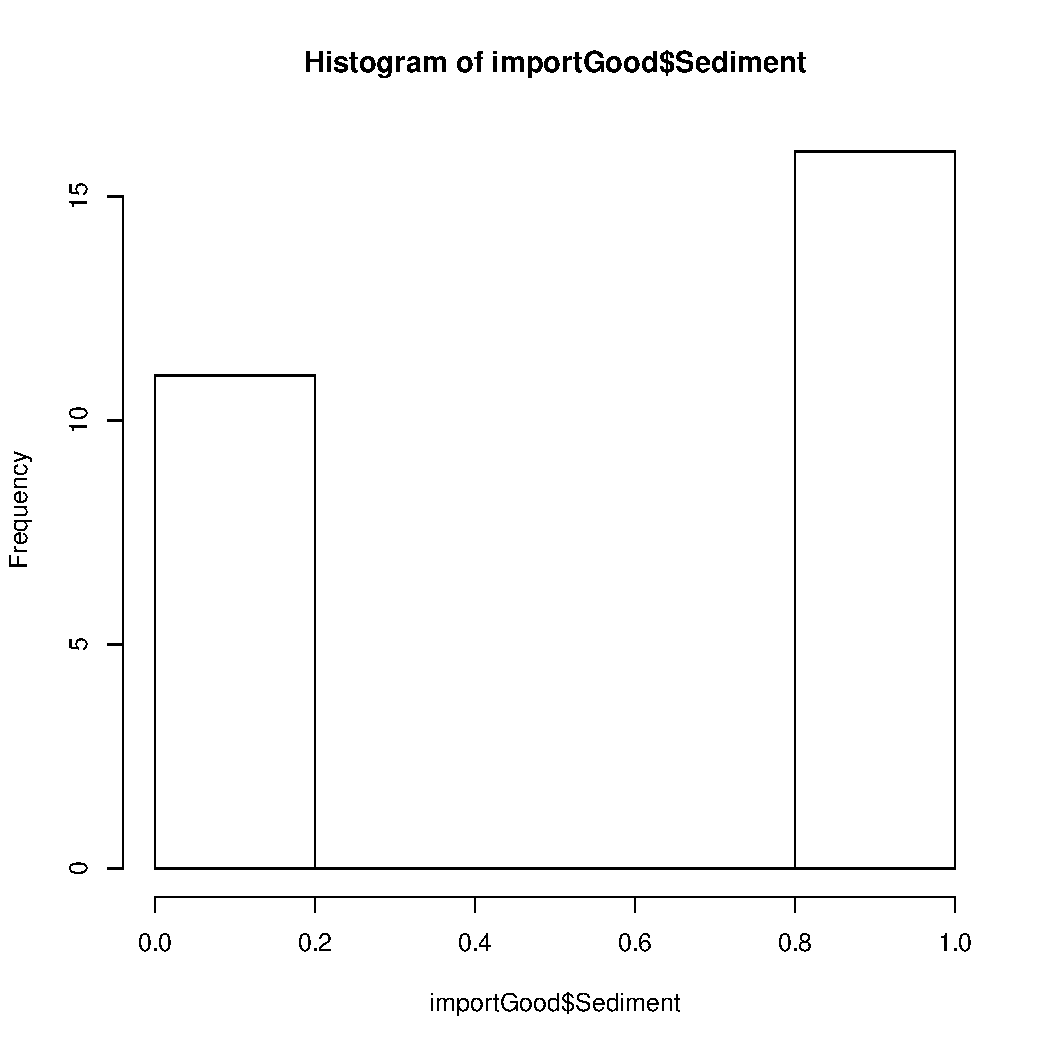
\includegraphics[width=\maxwidth]{figure/unnamed-chunk-4-1} 

\end{knitrout}

\begin{knitrout}
\definecolor{shadecolor}{rgb}{0.969, 0.969, 0.969}\color{fgcolor}\begin{kframe}
\begin{alltt}
\hlkwd{hist}\hlstd{(importGood}\hlopt{$}\hlstd{Temperature)}
\end{alltt}
\end{kframe}
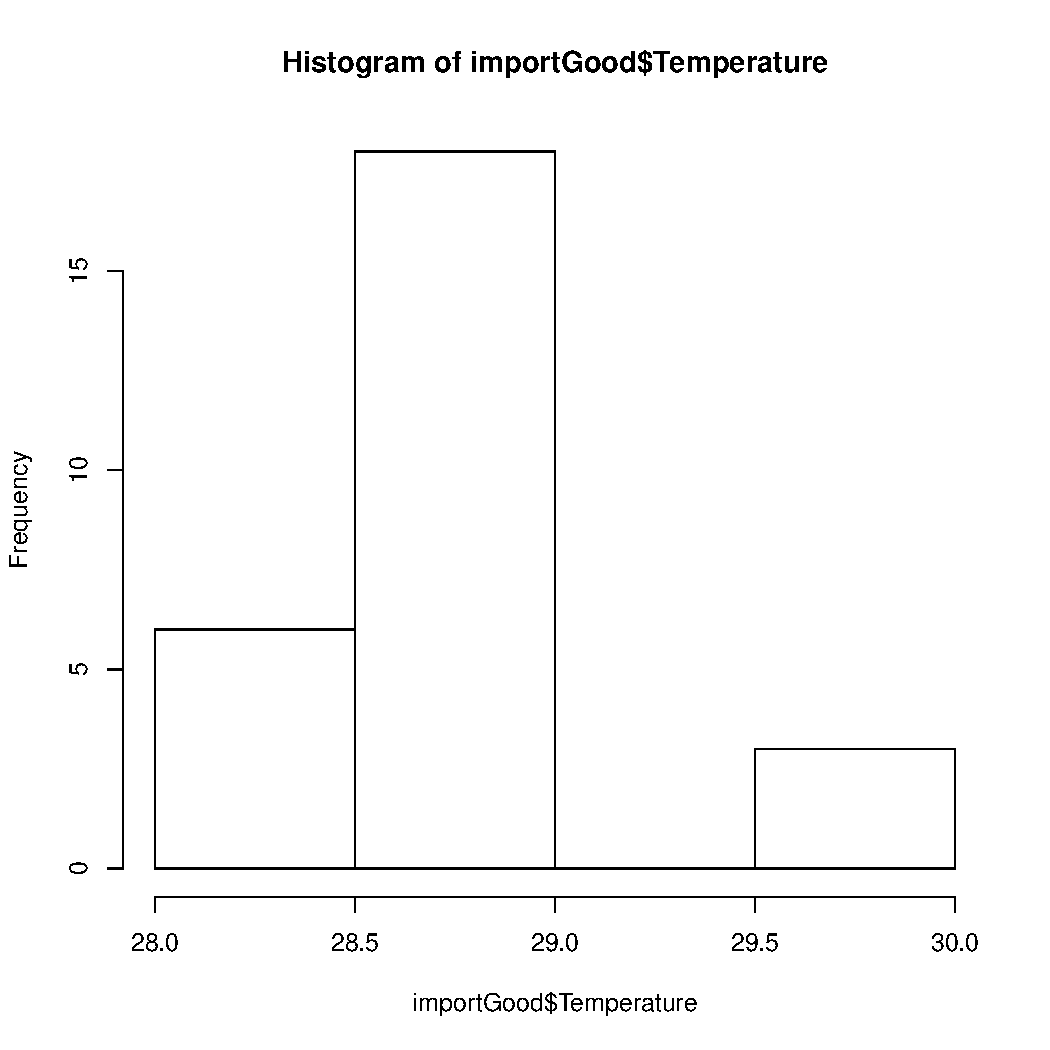
\includegraphics[width=\maxwidth]{figure/unnamed-chunk-5-1} 

\end{knitrout}


\begin{knitrout}
\definecolor{shadecolor}{rgb}{0.969, 0.969, 0.969}\color{fgcolor}\begin{kframe}
\begin{alltt}
\hlkwd{hist}\hlstd{(importGood}\hlopt{$}\hlstd{Canopy)}
\end{alltt}
\end{kframe}
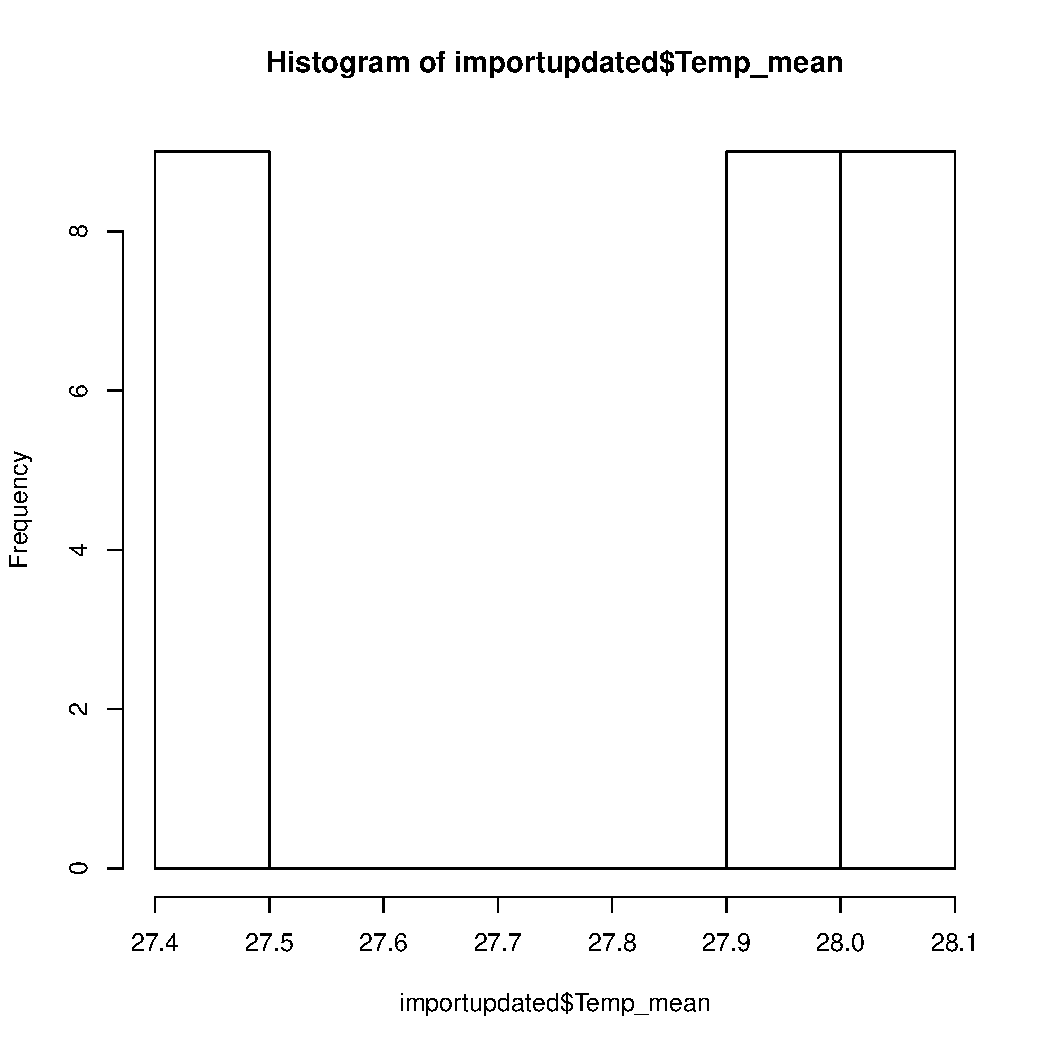
\includegraphics[width=\maxwidth]{figure/unnamed-chunk-6-1} 

\end{knitrout}

\section{Bias and Data Limitations}

All data collected on one day, Sept. 20, 2016.

Abnormal event (car accident) occurred a few ? days before data collection which caused the RIX treatment plant to temporarily shut off water outlet pipes, effectively draining the river and adeversely impacting algae populations to an unknown degree. Therefore our measurements likely reflect less-than-typical algae abundance. Our measuremnts were taken by undergraduate students without extensive algae fieldwork experience or training. 

\section{Results}

\begin{knitrout}
\definecolor{shadecolor}{rgb}{0.969, 0.969, 0.969}\color{fgcolor}\begin{kframe}
\begin{alltt}
\hlkwd{plot}\hlstd{(importGood}\hlopt{$}\hlstd{Temperature,importGood}\hlopt{$}\hlstd{Algae)}
\end{alltt}
\end{kframe}
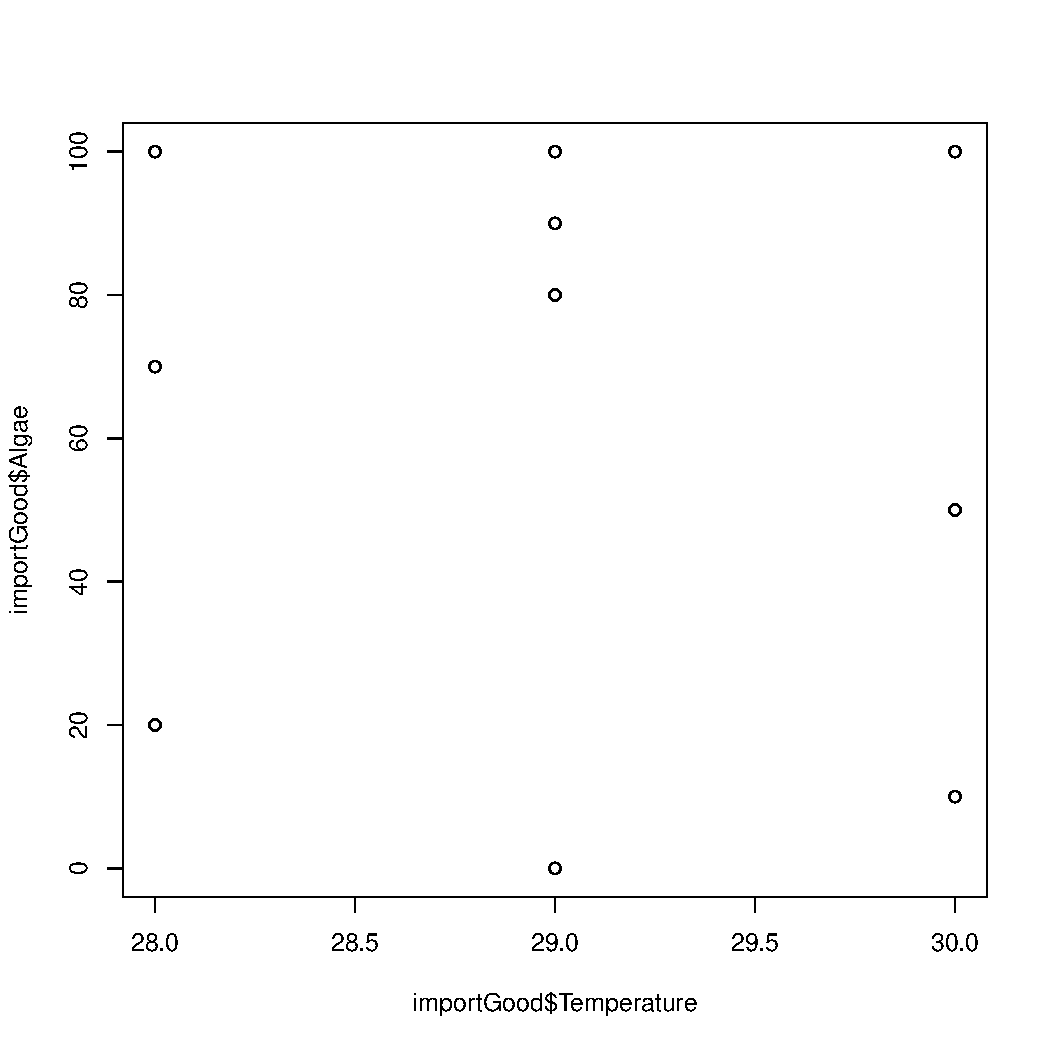
\includegraphics[width=\maxwidth]{figure/unnamed-chunk-7-1} 

\end{knitrout}
Our temperature data was too coarse to really be useful. Will eventually redo with other temp data, perhaps testing variance of temp by site rather than raw temp data. 
\begin{knitrout}
\definecolor{shadecolor}{rgb}{0.969, 0.969, 0.969}\color{fgcolor}\begin{kframe}
\begin{alltt}
\hlkwd{plot}\hlstd{(importGood}\hlopt{$}\hlstd{Canopy,importGood}\hlopt{$}\hlstd{Algae)}
\end{alltt}
\end{kframe}
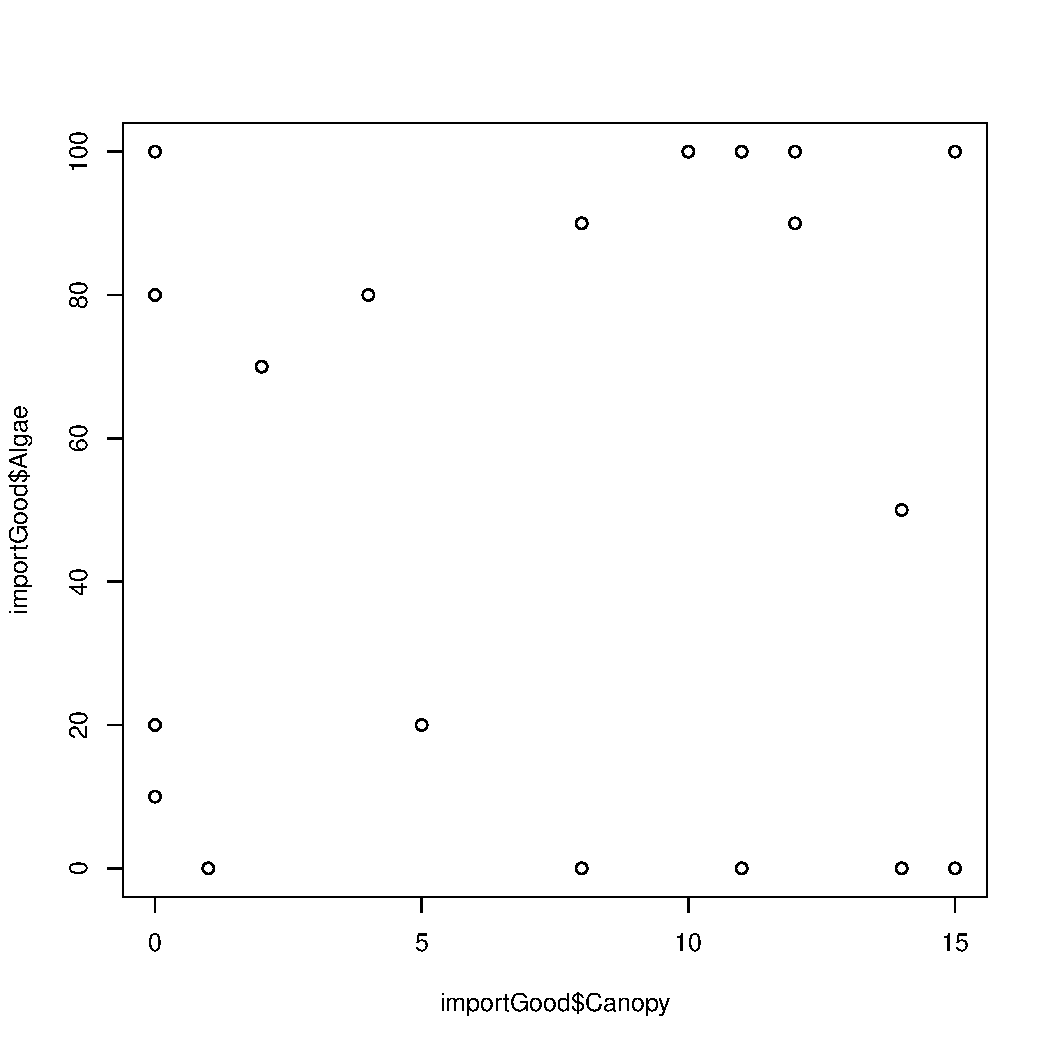
\includegraphics[width=\maxwidth]{figure/unnamed-chunk-8-1} 

\end{knitrout}
Cannot reject null hypothesis. 
\begin{knitrout}
\definecolor{shadecolor}{rgb}{0.969, 0.969, 0.969}\color{fgcolor}\begin{kframe}
\begin{alltt}
\hlkwd{plot}\hlstd{(importGood}\hlopt{$}\hlstd{Canopy,importGood}\hlopt{$}\hlstd{Temperature)}
\end{alltt}
\end{kframe}
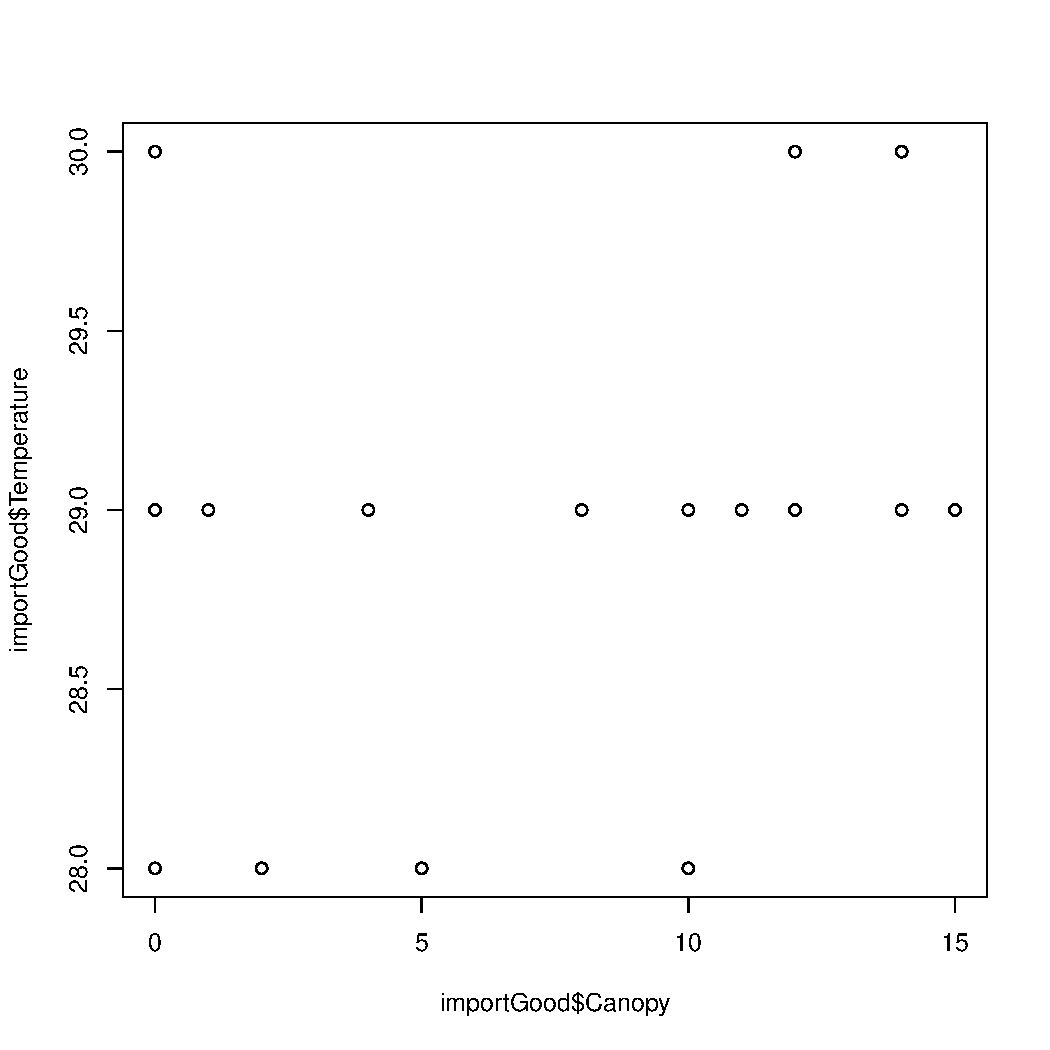
\includegraphics[width=\maxwidth]{figure/unnamed-chunk-9-1} 

\end{knitrout}
Our temperature data was too coarse to really be useful. Will eventually redo with other temp data, perhaps testing variance of temp by site rather than raw temp data. 
\begin{knitrout}
\definecolor{shadecolor}{rgb}{0.969, 0.969, 0.969}\color{fgcolor}\begin{kframe}
\begin{alltt}
\hlkwd{boxplot}\hlstd{(Algae}\hlopt{~}\hlstd{Sediment,importGood)}
\end{alltt}
\end{kframe}
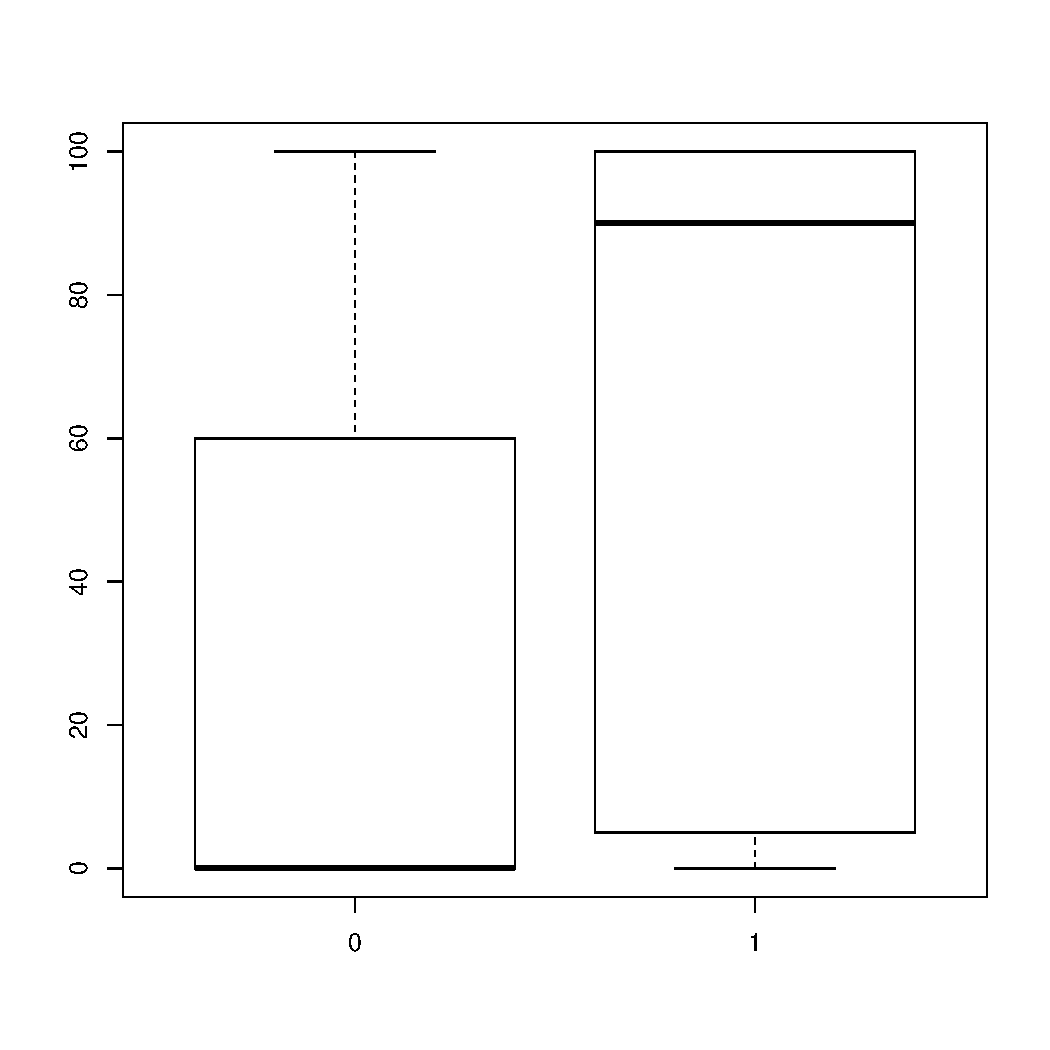
\includegraphics[width=\maxwidth]{figure/unnamed-chunk-10-1} 

\end{knitrout}
Our Pr(>F)=0.0643 which means we cannot reject null hypothesis, but only barely. This indicates that there is probably some relationship between algae cover and sediment composition of the stream bed, and this should be examined in future. hmmmm. 
\end{document}
